%==============================================================================
% Sjabloon poster bachproef
%==============================================================================
% Gebaseerd op document class `a0poster' door Gerlinde Kettl en Matthias Weiser
% Aangepast voor gebruik aan HOGENT door Jens Buysse en Bert Van Vreckem

\documentclass[a0,portrait]{hogent-poster}

% Info over de opleiding
\course{Bachelorproef}
\studyprogramme{toegepaste informatica}
\academicyear{2023-2024}
\institution{Hogeschool Gent, Valentin Vaerwyckweg 1, 9000 Gent}

% Info over de bachelorproef
\title{Authenticatie en Autorisatie in applicatieontwikkeling, hoe kan dit makkelijk worden aangeboden: Een diepgaande analyse en implementatie.}
% \subtitle{Ondertitel (eventueel)}
\author{Lander De Kesel}
\email{lander.dekesel@student.hogent.be}
\supervisor{Dhr. Gertjan Bosteels}
\cosupervisor{Dhr. Kris Van Opstaele (TrustBuilder)}

% Indien ingevuld, wordt deze informatie toegevoegd aan het einde van de
% abstract. Zet in commentaar als je dit niet wilt.
\specialisation{Mobile \& Enterprise development}
\keywords{Authenticatie, Autorisatie, Applicatieontwikkeling, Beveiliging, Privacy, RBAC, MFA}
\projectrepo{https://github.com/LanderDK/latex-hogent-bachproef-LanderDeKesel}

\begin{document}

\maketitle

\begin{abstract}
  In dit onderzoek wordt de implementatie van authenticatie en autorisatie in applicatieontwikkeling onder de loep genomen. 
  Door bestaande oplossingen en technologieën te analyseren en vergelijken, wordt gepoogd om praktische en eenvoudige oplossingen
  aan te bieden die de veiligheid waarborgen en de gebruikerservaring optimaliseren.
\end{abstract}

\begin{multicols}{2} % This is how many columns your poster will be broken into, a portrait poster is generally split into 2 columns


\section{Introductie}

In de hedendaagse digitale wereld zijn applicaties onmisbaar. Veiligheidsaspecten zoals authenticatie en autorisatie worden steeds 
belangrijker door de toename van digitale transacties en gegevensuitwisseling. Dit onderzoek richt zich op het vereenvoudigen van deze
processen en het bieden van praktische oplossingen voor ontwikkelaars.

\section{Probleemstelling}

De implementatie van veilige en gebruiksvriendelijke authenticatie en autorisatie is vaak complex en tijdrovend. Bestaande oplossingen zijn
vaak afhankelijk van externe diensten die beperkingen opleggen en kosten met zich meebrengen. Dit onderzoek analyseert en evalueert bestaande
oplossingen en technologieën om ontwikkelaars te helpen veilige applicaties te bouwen zonder afhankelijk te zijn van externe aanbieders.

\section{Onderzoeksvraag}

De centrale onderzoeksvraag is: ``Hoe kunnen ontwikkelaars effectieve en veilige authenticatie- en autorisatiesystemen implementeren in applicaties,
zonder afhankelijk te zijn van externe diensten of aanbieders, en tegelijkertijd een optimale gebruikerservaring bieden?''

\section{Onderzoeksdoelstelling}

Het doel van dit onderzoek is een grondige analyse van bestaande oplossingen en technologieën voor authenticatie en autorisatie. Het onderzoek
streeft ernaar om verbeteringen en aanpassingen voor te stellen die de uitdagingen en problemen van ontwikkelaars aanpakken.

\section{Methodologie}

De methodologie omvat een literatuurstudie van bestaande technologieën en een vergelijkende studie van veelbelovende aanbieders. De nadruk ligt
op het identificeren van pijnpunten en het doen van aanbevelingen voor verbeteringen op basis van concrete use cases.

\section{Resultaten}

Uit het onderzoek blijkt dat bestaande providers vaak beperkingen en kosten met zich meebrengen. Als alternatief kunnen ontwikkelaars kiezen voor
een zelfontwikkelde authenticatieserver die het OAuth 2.0 framework implementeert of gebruik maken van een Docker image van Keycloak on-premise.
  
\section{Sectie met figuur}

\begin{center}
  \captionsetup{type=figure}
  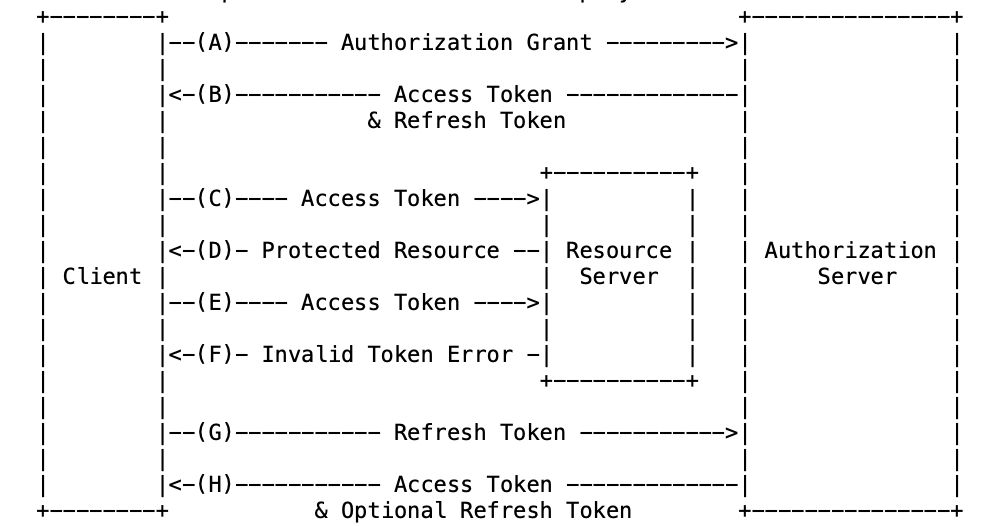
\includegraphics[width=1.0\linewidth]{graphics/oauth2.png}
  \captionof{figure}{OAuth 2.0 verloop}
\end{center}
\begin{center}
  \captionsetup{type=figure}
  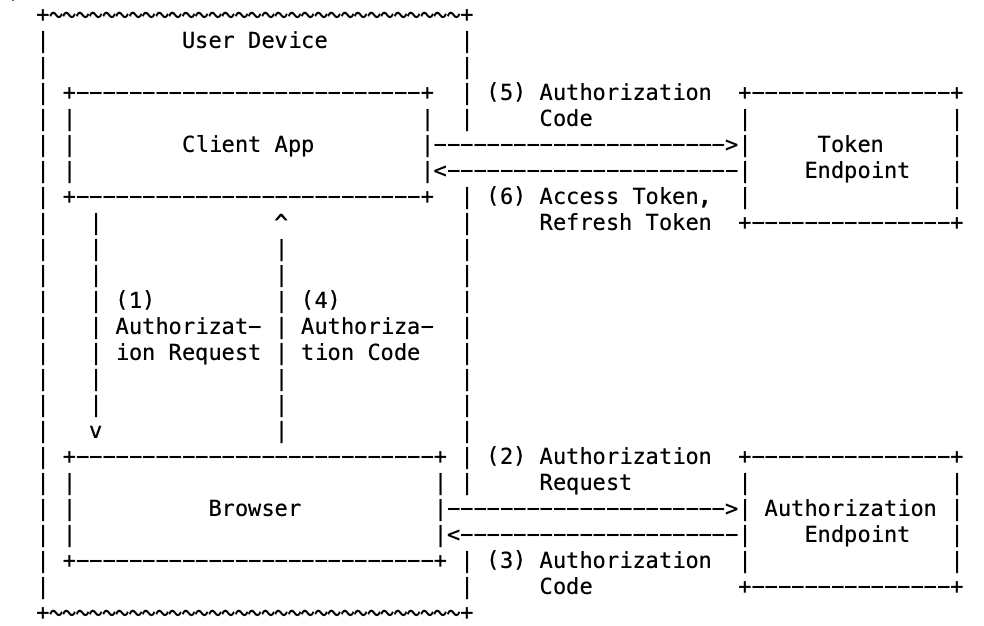
\includegraphics[width=1.0\linewidth]{graphics/oauth2_native.png}
  \captionof{figure}{OAuth 2.0 verloop in native apps}
\end{center}

\section{Conclusies}

Authenticatie en autorisatie zijn verder ontwikkeld dan aanvankelijk gedacht. Ontwikkelaars kiezen vaak voor bestaande providers, maar alternatieven
zoals Keycloak of een zelfontwikkelde server bieden kosten- en flexibiliteitsvoordelen. Verder onderzoek kan zich richten op het verbeteren van de
gebruikerservaring en het verlagen van kosten bij het gebruik van bestaande providers.

\section{Toekomstig onderzoek}

Toekomstig onderzoek kan zich richten op het verbeteren van de gebruikerservaring bij zelfontwikkelde authenticatieservers en het verlagen van kosten
bij het gebruik van bestaande providers. Dit onderzoek biedt een startpunt voor ontwikkelaars om geïnformeerde beslissingen te nemen over authenticatie-
en autorisatieoplossingen.

\section{Referenties}
\begin{itemize}
    \item Denniss, W., \& Bradley, J. (2017). OAuth 2.0 for Native Apps. \textit{RFC 8252}. Retrieved from \url{https://www.rfc-editor.org/info/rfc8252}
    \item Hardt, D. (2012). The OAuth 2.0 Authorization Framework. \textit{RFC 6749}. Retrieved from \url{https://www.rfc-editor.org/info/rfc6749}
    \item Sheffer, Y., Hardt, D., \& Jones, M. B. (2020). JSON Web Token Best Current Practices. \textit{RFC 8725}. Retrieved from \url{https://www.rfc-editor.org/info/rfc8725}
    \item Sakimura, N., Bradley, J., Jones, M., De Medeiros, B., \& Mortimore, C. (2014). OpenID Connect Core 1.0 incorporating errata set 1. \textit{The OpenID Foundation, Specification, 335}. Retrieved from \url{https://openid.net/specs/openid-connect-core-1_0.html}
\end{itemize}

\end{multicols}
\end{document}